\chapter{Реализация программы с использованием библиотеки MNE}
\label{ch:chap1}

    Программа осуществляет чтение данных электроэнцефалограммы (ЭЭГ), выполняет их анализ для выявления артефактов, а затем устраняет их с использованием фильтров с конечной импульсной характеристикой (КИХ), построенных на основе окна Хэмминга. В частности, для удаления низкочастотных дрейфов применяется высокочастотный КИХ-фильтр, а для подавления сетевых и других узкополосных помех используется узкополосный режекторный КИХ-фильтр, также реализованный с использованием окна Хэмминга.

    После предварительной обработки данных осуществляется построение топографических карт электрической активности головного мозга за заданный временной интервал. Полученные изображения сохраняются для дальнейшего анализа и обработки, что позволяет исследовать пространственное распределение активности мозга и выявлять ключевые паттерны в данных.

\section{Считывание данных и их первичный анализ}
    На данном этапе производится считывание данных их исследоавание на наличие различного рода помех.
    \begin{enumerate}
        \item Считывание ЭЭГ-данных
        \item Визуальное представление считанных
        \begin{enumerate}
            \item Построение графика временного ряда данных для всех датчиков
            \item Построение графика спектральной плотности мощности сигнала (СПМ)
        \end{enumerate}
        \item Выявление помех
        \begin{enumerate}
            \item Низкочастотных дрейфов
            \item Узкополосных помех
        \end{enumerate}
    \end{enumerate}

\section{Предобработка данных}

Предобработка ЭЭГ данных включает в себя несколько ключевых этапов, направленных на улучшение качества сигналов и снижение влияния помех, что критически важно для дальнейшего анализа и интерпретации результатов. Этот процесс состоит из следующих шагов:
\begin{enumerate}
\item \textbf{Фильтрация.}
\newline
ЭЭГ-сигналы подвержены различным высокочастотным и низкочастотным помехам, таким как шумы от электроприборов, мышечных артефактов и дыхания. Для удаления нежелательных частот применяют фильтрацию.
В частности, в данной программе была примененен высокочастотный КИХ-фильтр, построенный на основе окна Хэмминга, для удаления низкочастотных дрейфов.

В данном фильтре фильтрация временного ряда выполняется с помощью свёртки исходного сигнала \(x[n]\) с импульсной характеристикой фильтра \(h[k]\). Формула фильтрации имеет вид:

\begin{equation}
y[n] = \sum_{k=0}^{M} h[k] \cdot x[n-k], \quad n = M, \dots, N-M,
\label{eq:fir_filter}
\end{equation}

где:
\begin{itemize}
    \item \(y[n]\) — выходной (отфильтрованный) сигнал,
    \item \(x[n]\) — входной сигнал,
    \item \(h[k]\) — импульсная характеристика фильтра,
    \item \(M\) — длина фильтра,
    \item \(N\) — длина входного сигнала.
\end{itemize}

Для сглаживания коэффициентов фильтра используется окно Хэмминга, определяемое следующим образом:

\begin{equation}
w[k] = 0.54 - 0.46 \cos\left( \frac{2 \pi k}{M} \right), \quad k = 0, \dots, M.
\label{eq:hamming_window}
\end{equation}

Импульсная характеристика высокочастотного фильтра с частотой отсечки \(f_c\) задаётся как:

\begin{equation}
h[k] = w[k] \cdot \left( \delta[k] - \frac{\sin(2 \pi f_c (k - M/2))}{\pi (k - M/2)} \right), \quad k = 0, \dots, M,
\label{eq:filter_kernel}
\end{equation}

где:
\begin{itemize}
    \item \(\delta[k]\) — дельта-функция (единица при \(k = M/2\), иначе ноль),
    \item \(f_c\) — частота отсечки в долях от частоты дискретизации,
    \item \(w[k]\) — окно Хэмминга (см. формулу \eqref{eq:hamming_window}).
\end{itemize}

\item \textbf{Удаление артефактов.}
\newline
Одними из основных источников помех являются движения глаз, миографические артефакты и электрические помехи от окружающих устройств. Для их устранения применяются различные методы,
В данной программе точечно применяется узкополосной режекторный КИХ-фильтр для подавления узкополосных миографических помех.

Фильтрация сигнала выполняется через свёртку входного сигнала \(x[n]\) с импульсной характеристикой фильтра \(h[k]\):

\begin{equation}
y[n] = \sum_{k=0}^{M} h[k] \cdot x[n-k], \quad n = M, \dots, N-M,
\label{eq:notch_filter}
\end{equation}

где:
\begin{itemize}
    \item \(y[n]\) — выходной (отфильтрованный) сигнал,
    \item \(x[n]\) — входной сигнал,
    \item \(h[k]\) — импульсная характеристика фильтра,
    \item \(M\) — длина фильтра,
    \item \(N\) — длина входного сигнала.
\end{itemize}

Импульсная характеристика полосозаградительного фильтра задаётся следующим образом:

\begin{equation}
\begin{split}
h[k] &= w[k] \cdot \left( \delta[k] - \frac{\sin(2 \pi f_1 (k - M/2))}{\pi (k - M/2)} + \frac{\sin(2 \pi f_2 (k - M/2))}{\pi (k - M/2)} \right), \\
& \quad k = 0, \dots, M
\end{split}
\end{equation}

где:
\begin{itemize}
    \item \(w[k]\) — окно Хэмминга, задаваемое формулой \eqref{eq:hamming_window},
    \item \(\delta[k]\) — дельта-функция (единица при \(k = M/2\), иначе ноль),
    \item \(f_1\) и \(f_2\) — границы вырезаемой полосы в долях от частоты дискретизации (\(f_1 = f - \text{trans\_bandwidth}\), \(f_2 = f + \text{trans\_bandwidth}\)),
    \item \(M\) — длина фильтра.
\end{itemize}

Для сглаживания переходов в частотной характеристике фильтра применяется окно Хэмминга, определяемое как:

\begin{equation}
w[k] = 0.54 - 0.46 \cos\left( \frac{2 \pi k}{M} \right), \quad k = 0, \dots, M.
\label{eq:hamming_window}
\end{equation}

\item \textbf{Сегментация.}
\newline
Этап сегментации заключается в разбиении непрерывного сигнала на короткие фрагменты или эпизоды для дальнейшего анализа. Это позволяет сосредоточиться на интересующих участках данных, таких как стимулы, реакции или события.
В данной программе сегментация реализована посредством генерации топографических карт по заданному временому и частотному интервалам. После чего, вышеупомянутые карты сохраняются в формате PNG
\end{enumerate}
\newpage
Примеры временных срезов топографических карт для соответствующих каналов: \newline
\begin{figure}[!ht]
    \centering
    \begin{tabular}{cc}
        \begin{subfigure}[c]{0.3\textwidth}
            \centering
            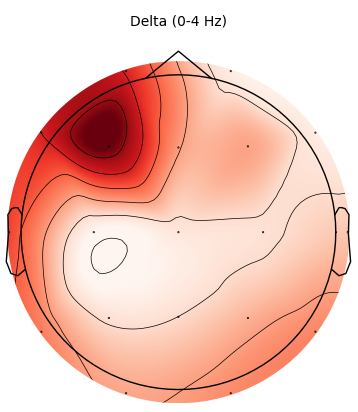
\includegraphics{images/topomap_delta_colored.png}
            \caption{}
        \end{subfigure}
        &
        \begin{subfigure}[c]{0.3\textwidth}
            \centering
            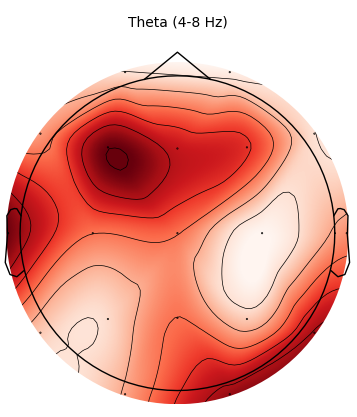
\includegraphics{images/topomap_theta_colored.png}
            \caption{}
        \end{subfigure}
    \end{tabular}
    \vspace{\abovecaptionskip}
    \begin{tabular}{ccc}
        \begin{subfigure}[c]{0.3\textwidth}
            \centering
            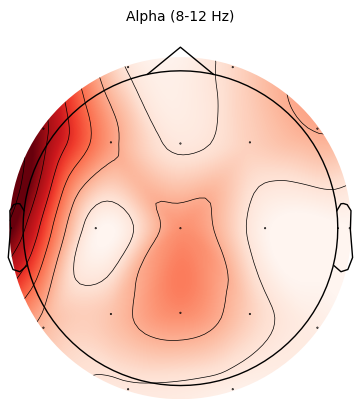
\includegraphics{images/topomap_alpha_colored.png}
            \caption{}
        \end{subfigure}
        &
        \begin{subfigure}[c]{0.3\textwidth}
            \centering
            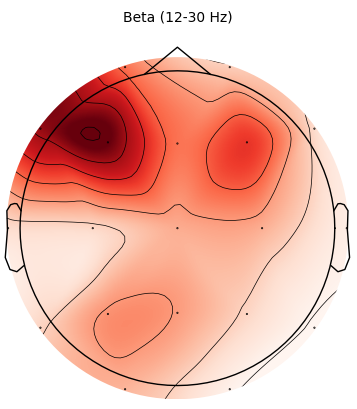
\includegraphics{images/topomap_beta_colored.png}
            \caption{}
        \end{subfigure}
        &
        \begin{subfigure}[c]{0.3\textwidth}
            \centering
            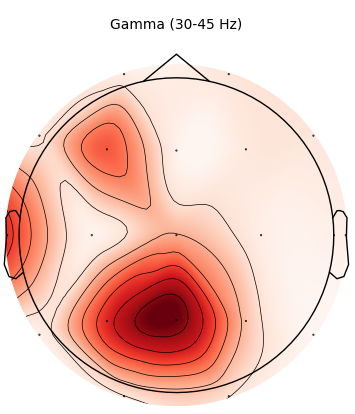
\includegraphics{images/topomap_gamma_colored.png}
            \caption{}
        \end{subfigure}
    \end{tabular}
    \caption{Топографические карты построенные по соответствующим каналам. (а) - Delta-канал (0-4 Гц), (б) - Theta-канал (4-8 Гц), (в) - Alpha-канал (8-12 Гц), (г) - Beta-канал (12-30 Гц), (д) - Gamma-канал (30-45 Гц),}
    \label{fig:topomap_colored}
\end{figure}

Задача предобработки заключается в улучшении качества ЭЭГ-сигналов, для корректного последующего анализа, включая извлечение характеристик, таких как альфа- и бета-ритмы. Недостаточная предобработка может привести к искажению результатов и ошибочным выводам, поэтому этот этап является обязательным в исследовательской практике.

\endinput